\chapter{Initial Framework: Foundational System and Baseline Evaluations}
\label{Chapter4}
\lhead{Chapter 4. \emph{Initial Framework and Baseline Evaluations}}

\section{Overview}

The foundational phase of this research established a functional prototype of a multi-agent clinical simulation using open-source language models. The system was governed by an ad-hoc \texttt{while}-loop architecture that sequentially routed requests among the Doctor, Patient, and Measurement agents. The primary objective was to assess whether relatively small, locally hosted LLMs (7B--8B parameters) could navigate a multi-turn diagnostic conversation and produce a recognisable disease prediction---a question that remained largely unanswered for open-source models at the time.

Figure~\ref{fig:agent-flowchart} illustrates the overall structure and information flow of the multi-agent clinical simulation framework. The diagram highlights how each agent interacts with the others through the Interaction Orchestrator, and how diagnostic reasoning emerges through sequential doctor--patient dialogue, structured test retrieval, and final moderator-based evaluation.

\begin{figure}[H]
    \centering
    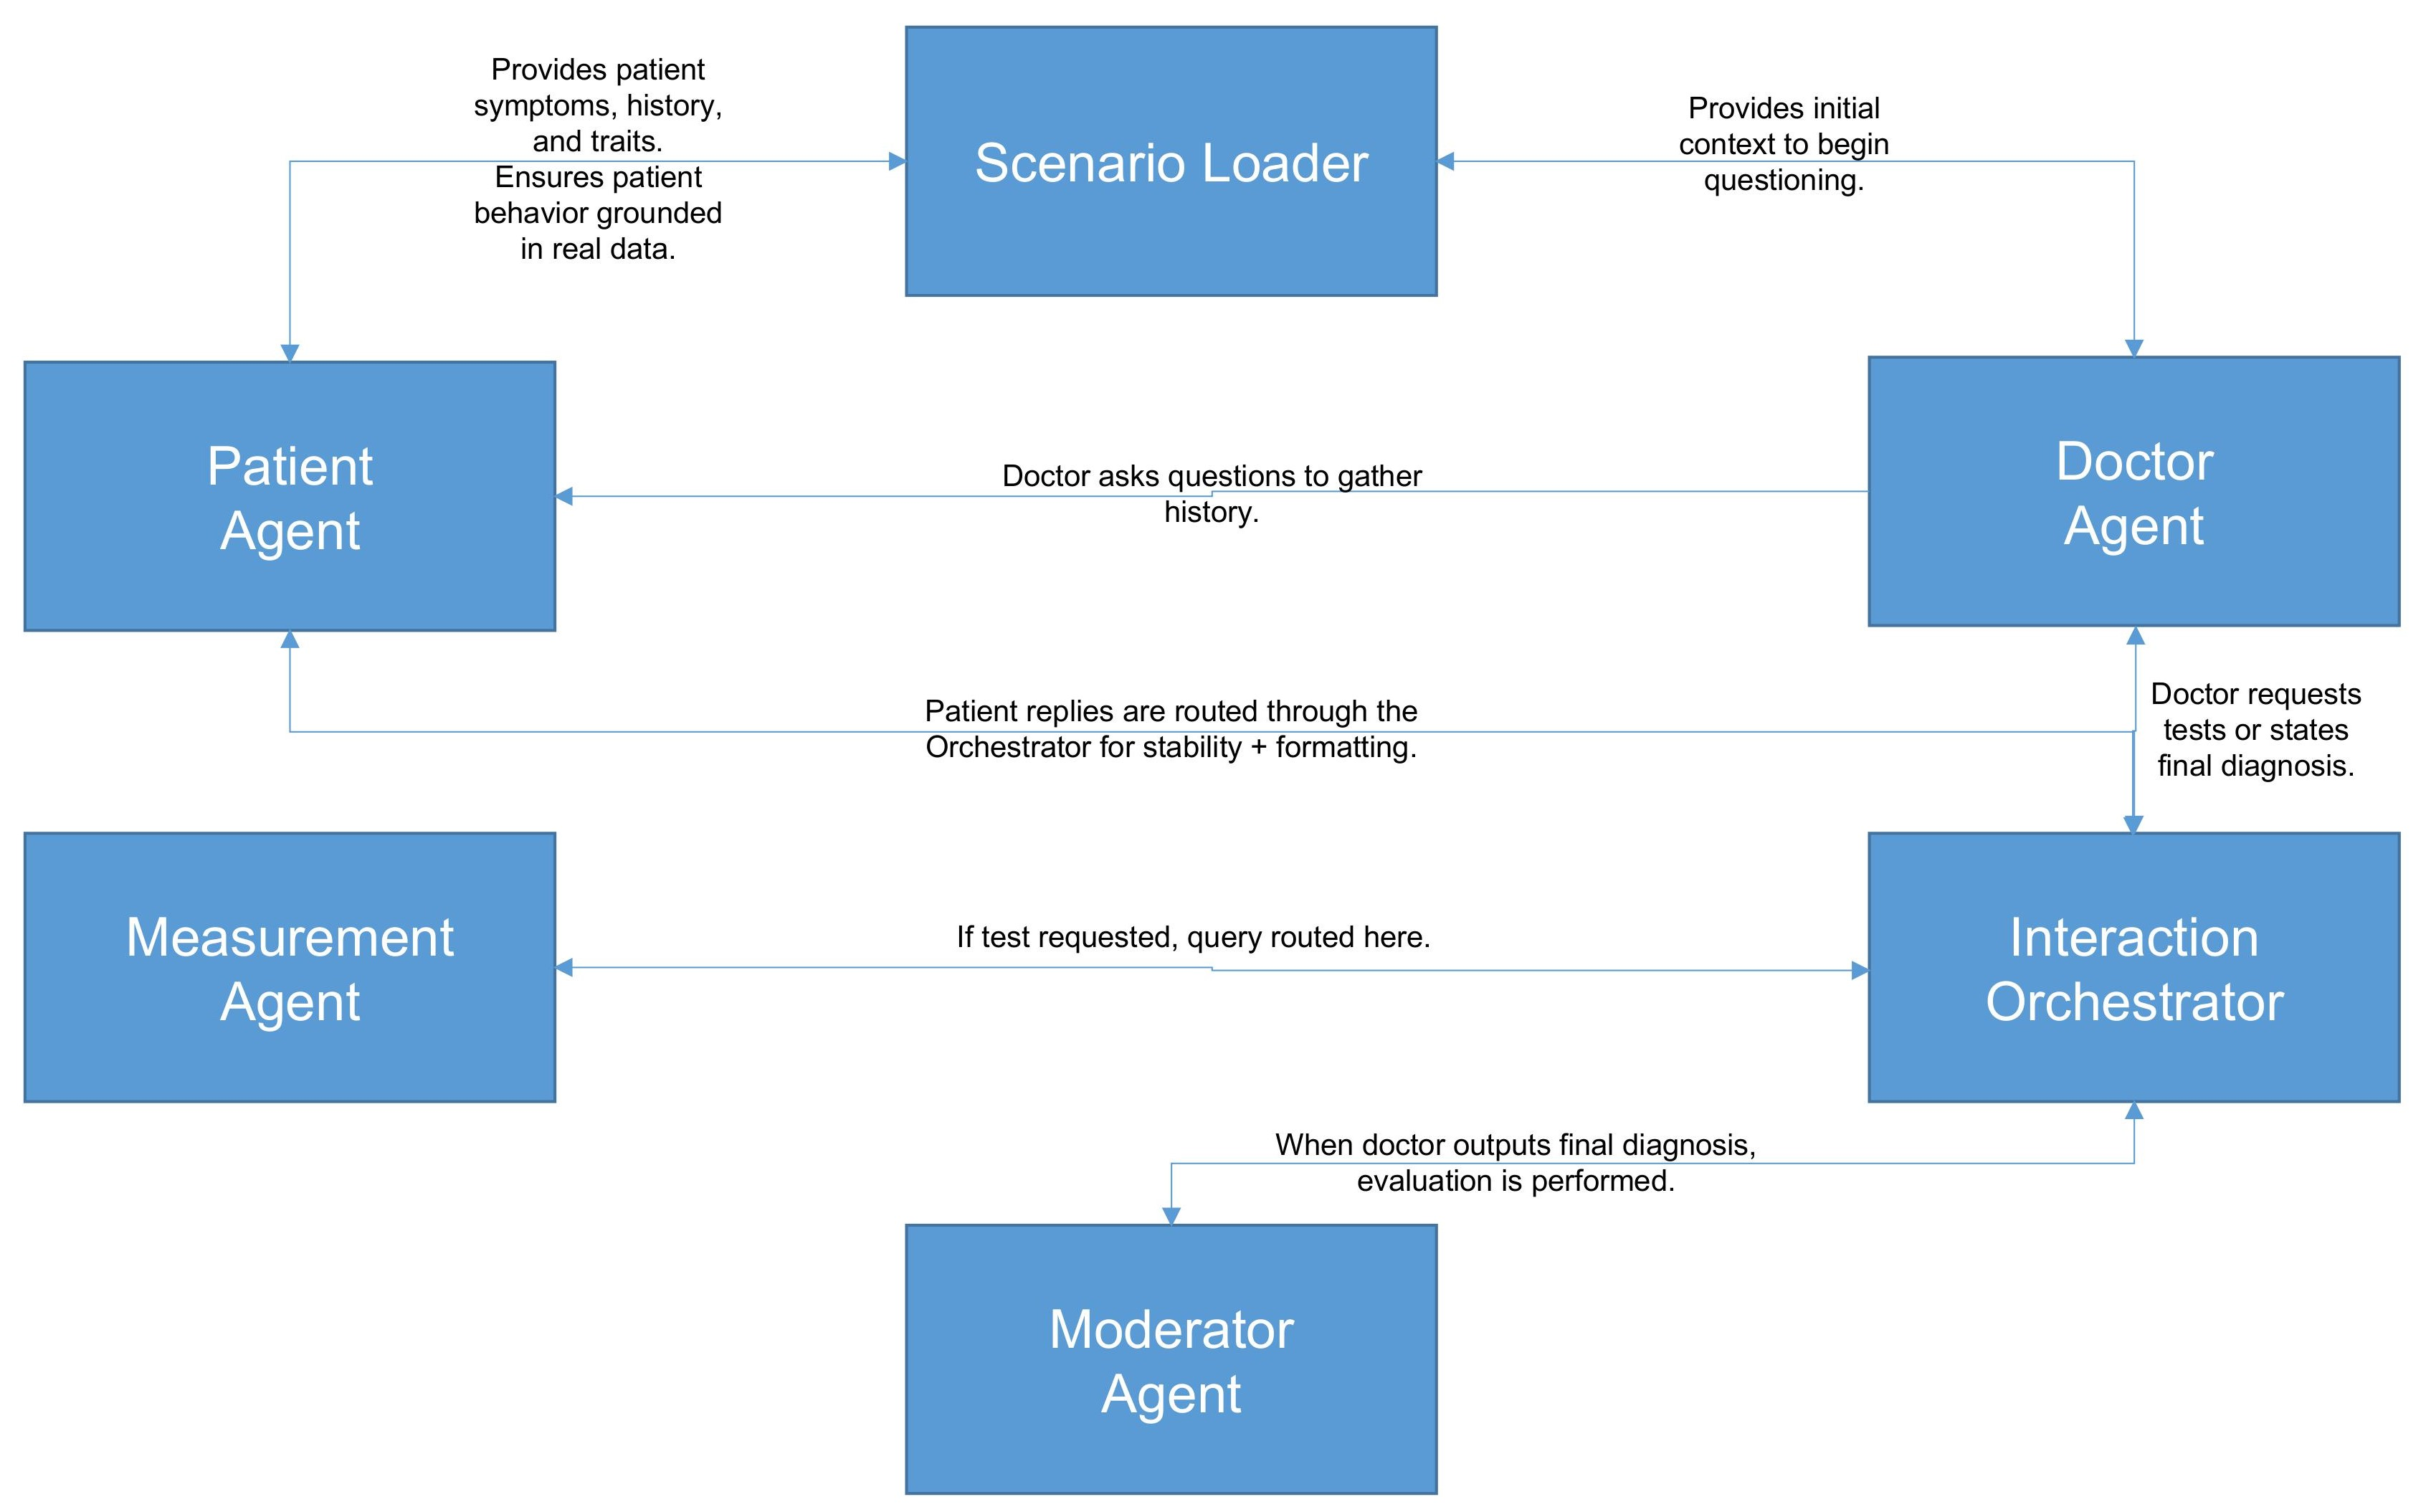
\includegraphics[width=\textwidth]{Pictures/Flowchart_pic.jpg}
    \caption{Overview of the multi-agent interaction workflow used in the clinical simulation framework. The Scenario Loader initializes each case and distributes case-specific information to the appropriate agents. The Doctor Agent performs history-taking, hypothesis generation, and test ordering. The Patient Agent produces symptom-grounded responses, while the Measurement Agent returns structured diagnostic tests upon request. All communication flows through the Interaction Orchestrator, which ensures turn-taking and state management. Once the Doctor provides a final diagnosis, the Moderator Agent evaluates its correctness through semantic comparison.}
    \label{fig:agent-flowchart}
\end{figure}

\section{Evaluated Models}

Four open-source models were selected, representing a spectrum from general-purpose instruction-tuning to narrow biomedical specialisation:
\begin{itemize}
    \item \textbf{Mistral-7B-Instruct-v0.2:} A strong general-purpose instruction-tuned model trained on diverse text corpora.
    \item \textbf{Microsoft BioGPT (1.5B):} A model pre-trained specifically on PubMed abstracts and biomedical literature.
    \item \textbf{JSL-Med-Sft-Llama-3-8B:} A Llama-3 derivative fine-tuned by John Snow Labs on clinical and biomedical datasets.
    \item \textbf{Apollo (7B):} A general-purpose baseline trained on broad web and text corpora without medical specialisation.
\end{itemize}

\section{Diagnostic Accuracy Results}

\subsection{Diagnostic Accuracy Calculation}

Diagnostic correctness is determined for each scenario by the Moderator Agent, which compares the Doctor Agent's final prediction against the scenario's ground truth. The overall accuracy is calculated as the ratio of correctly diagnosed cases to the total number of evaluated scenarios:
\[
\text{Accuracy} = \frac{\text{Number of Correct Diagnoses}}{\text{Total Number of Scenarios}} \times 100
\]
This constitutes the primary quantitative metric evaluating the baseline framework.

\subsection{Model Performances}

The models were tasked with diagnosing cases from the AgentClinic-MedQA subset. Table~\ref{tab:phase1_acc} and Figure~\ref{fig:phase1_acc} illustrate the diagnostic accuracy achieved.

\begin{table}[H]
\centering
\caption{Diagnostic accuracy of open-source LLMs on the AgentClinic-MedQA subset (initial framework).}
\label{tab:phase1_acc}
\begin{tabular}{@{}llc@{}}
\toprule
\textbf{Model} & \textbf{Training Data Alignment} & \textbf{Accuracy (\%)} \\ \midrule
Mistral-7B-Instruct-v0.2 & General instruction-tuning & 44.0 \\
Microsoft BioGPT         & Biomedical literature       & 35.0 \\
JSL-Med-Sft-Llama-3      & Clinical + Biomedical SFT   & 32.0 \\
Apollo                   & General text corpora        & 23.0 \\
\bottomrule
\end{tabular}
\end{table}

\begin{figure}[H]
\centering
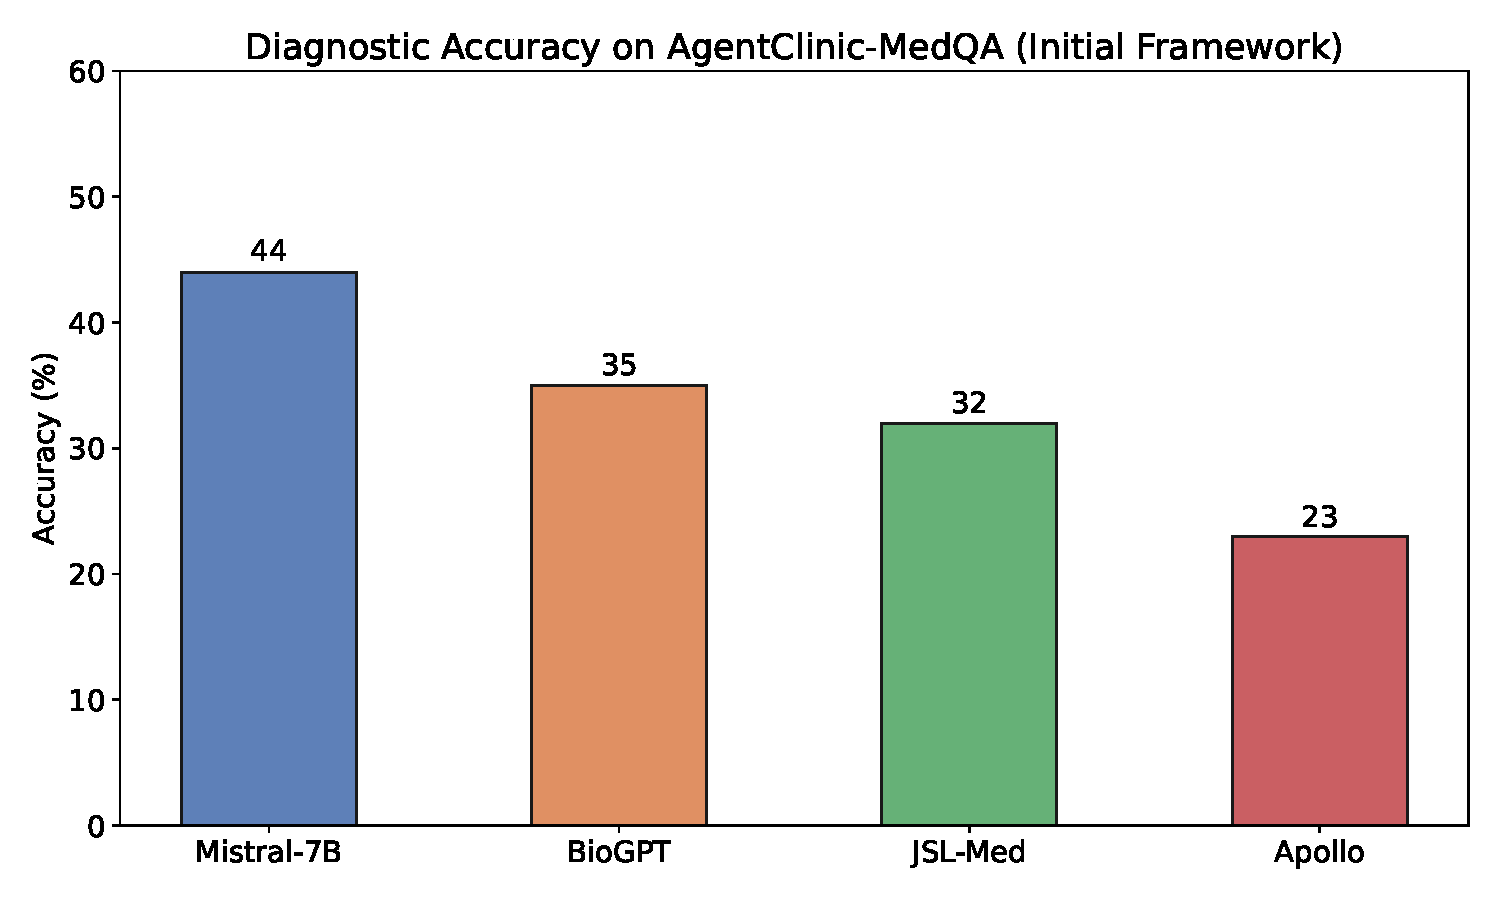
\includegraphics[width=\textwidth]{Pictures/phase1_acc.pdf}
\caption{Baseline diagnostic accuracy of open-source LLMs in the initial simulation framework. Paradoxically, the generalist Mistral-7B-Instruct-v0.2 outperformed all medically fine-tuned models.}
\label{fig:phase1_acc}
\end{figure}

The counter-intuitive result that a generalist model (Mistral-7B at 44\%) outperformed medically fine-tuned models (BioGPT at 35\%, JSL-Med at 32\%) highlighted a critical phenomenon: \textit{catastrophic forgetting}. Medical fine-tuning datasets are often narrow in scope. Optimising for these narrow tasks erodes the models' broad conversational logic and instruction-following capabilities required to navigate a multi-turn interactive simulation, resulting in degraded performance despite superior declarative medical knowledge.

\section{Bias Impact Analysis}

Preliminary, prompt-based bias injections were implemented to observe performance degradation in the best-performing model (Mistral-7B at 44\% unbiased accuracy). The following cognitive and demographic biases were introduced:
\begin{itemize}
    \item \textbf{Recency Bias:} Accuracy dropped to 34\%.
    \item \textbf{Gender Bias (Implicit):} Accuracy dropped to 35\%.
    \item \textbf{Confirmation Bias:} Accuracy dropped to 32\%.
\end{itemize}

These results confirmed that cognitive and demographic biases systematically degrade LLM diagnostic accuracy. Confirmation bias caused the greatest degradation, as the model became anchored to an initial incorrect hypothesis and selectively amplified supporting evidence while discounting contradictory symptoms.

\section{Identified Architectural Limitations}

While the initial prototype was successfully implemented, severe structural flaws were identified which motivated the complete system redesign:

\begin{enumerate}
    \item \textbf{Non-Deterministic Execution:} The \texttt{while}-loop frequently failed to correctly handle agent transitions when the LLM generated malformed stop tokens, leading to simulation crashes or silent skips.
    \item \textbf{Absence of Trajectory Analysis:} Only terminal outcomes were measured. A model that guessed correctly without ordering any diagnostic tests received an identical score to a methodical, evidence-driven clinician.
    \item \textbf{Lexical Leakage Vulnerability:} Due to VRAM constraints, a \textit{homogeneous engine} was employed: the same Mistral-7B weights generated both the patient's symptoms and the doctor's diagnosis. Theoretical analysis revealed that these shared model weights cause both agents to project text into identical latent embedding manifolds. The Doctor agent may therefore subconsciously ``recognise'' the mathematical structure of the Patient's generated text, gaining implicit access to ground-truth information---a phenomenon formalised in this thesis as \textbf{Lexical Leakage}.
\end{enumerate}

These limitations collectively motivated the development of AgentClinic~v2.1, described in the following chapter.
